% TODO: Choose thesis language.
\documentclass[estonian,english]{unitartucs-thesis} % Thesis is in English, but info page also has Estonian.
% \documentclass[english,estonian]{unitartucs-thesis} % Thesis is in Estonian, but info page also has English.

% Modern encoding, do not remove.
\usepackage[utf8]{inputenc}
\usepackage[T1]{fontenc}

% Bibliography with BibLaTeX.
% TODO: Choose citation and bibliography style.
\usepackage[style=unitartucs-numeric]{biblatex} % Numeric citations [1], alphabetically sorted bibliography.
% \usepackage[style=unitartucs-numeric,sorting=none]{biblatex} % Numeric citations [1], bibliography in citation order.
% \usepackage[style=unitartucs-alphabetic]{biblatex} % Alphabetic citations [ABC], alphabetically sorted bibliography.

\DeclareLanguageMapping{english}{unitartucs-english} % Language overrides for english.
\DeclareLanguageMapping{estonian}{unitartucs-estonian} % Language overrides for estonian.
\addbibresource{thesis.bib} % Bibliography file itself.

% Packages for math.
\usepackage{amsmath}
\usepackage{amssymb} % Package for additional math symbols.
\usepackage{amsthm} % Package for theorems, definitions, etc.
\theoremstyle{plain}
\newtheorem{theorem}{Theorem} % TODO: Translate to Teoreem if thesis is in Estonian.
\theoremstyle{definition}
\newtheorem{definition}{Definition} % TODO: Translate to Definitsioon if thesis is in Estonian.

% Package for graphics/images.
\usepackage{graphicx}
\graphicspath{{figures/}} % Directory of graphics.

\usepackage{booktabs} % Package for nice and professional tables (\toprule, \midrule, \bottomrule).
\usepackage{subcaption} % Package for subfigures and subtables.

% Package for source code.
\usepackage{minted}
\setminted{autogobble} % Trim common leading whitespace from code.

\usepackage{xspace} % Non-eatable spaces in macros
% Define your favorite macros that you use inside the thesis
% Name followed by non-removable space
\newcommand{\proveit}{ProveIt\xspace}

% Package for TODO notes with \todo command.
\usepackage{todonotes}
\newcommand{\TODO}{\todo[inline]} % Custom command for inline TODOs.


% TODO: Fill in title and author name.
\title{Type Inference for Fourth Order Logic Formulae}
\author{Alice Cooper}

% TODO: Fill in supervisors. Use \and to separate multiple supervisors. Use \degree to specify their degree.
\supervisor{Axel Rose\degree{MSc} \and May Flower\degree{PhD}}

% TODO: Choose curriculum.
\curriculum{Computer Science Curriculum}
% \curriculum{Software Engineering Curriculum}
% \curriculum{Informaatika õppekava}

% TODO: Choose thesis type (bachelor's or master's) and number of ECTS.
\thesis{Master's Thesis (30 ECTS)}
% \thesis{Bakalaureusetöö (9 EAP)}
% \thesis{Bachelor's Thesis (9 ECTS)}

% Override year (on title page) and date (in licence). Defaults to today.
% \date{2023-01-02}


\appto\biburlsetup{\Urlmuskip=0mu\relax} % https://tex.stackexchange.com/a/291857
\begin{document}

\maketitle % Title page
\newpage
\pdfbookmark[section]{\infoname}{info} % Add info page to PDF bookmarks (for convenience), but not to Table of Contents.

% Info in main language.
\begin{info}
\begin{abstract}
% TODO: Add abstract.
Many interpreting program languages are dynamically typed, such as Visual Basic or Python. As a result, it is easy to write programs that crash due to mismatches of provided and expected data types.  One possible solution to this problem is automatic type derivation during compilation. In this work, we consider study how to detect type errors in the \textsc{Whitespace} language by using fourth-order logic formulae as annotations. The main result of this thesis is a new triple-exponential type inference algorithm for the fourth-order logic formulae. This is a significant advancement as the question of whether there exists such an algorithm was an open question.
All previous attempts to solve the problem lead to logical inconsistencies or require tedious user interaction in terms of interpretative dance. Although the resulting algorithm is slightly inefficient, it can be used to detect obscure programming bugs in the \textsc{Whitespace} language. The latter significantly improves productivity. Our practical experiments showed that productivity is comparable to average Java programmer.
From a theoretical viewpoint, the result is only a small advancement in a rigorous treatment of higher-order logic formulae. The results obtained by us do not generalise to formulae with the fifth or higher order.
\end{abstract}

% TODO: Add keywords, separated by commas.
\keywords{\TODO{List of keywords}}

\cercs{\TODO{CERCS code and name:~\url{https://www.etis.ee/Portal/Classifiers/Details/d3717f7b-bec8-4cd9-8ea4-c89cd56ca46e}}}
\end{info}


% Info in other language.
% TODO: Choose other language (estonian or english).
% TODO: Fill in title in other language.
\begin{otherinfo}{estonian}{Tüübituletus neljandat järku loogikavalemitele}
\begin{abstract}
% TODO: Add abstract in other language.
\TODO{One or two sentences providing a basic introduction to the field, comprehensible to a scientist in
any discipline.}
\TODO{Two to three sentences of
more detailed background, comprehensible to scientists in related disciplines.}
\TODO{One sentence clearly stating the general problem being addressed by this particular
study.}
\TODO{One sentence summarising the main result (with the words ``here we show´´ or their equivalent).}
\TODO{Two or three sentences explaining what
the main result reveals in direct
comparison to what was thought to be the case previously, or how the main result adds to previous knowledge.}
\TODO{One or two sentences to put the results into a more general context.}
\TODO{Two or three sentences to provide a
broader perspective, readily
comprehensible to a scientist in any
discipline, may be included in the first paragraph
if the editor considers that the accessibility of
the paper is significantly enhanced by their inclusion.}
\end{abstract}

% TODO: Add keywords in other language, separated by commas.
\keywords{\TODO{List of keywords}}

\cercs{\TODO{CERCS kood ja nimetus:~\url{https://www.etis.ee/Portal/Classifiers/Details/d3717f7b-bec8-4cd9-8ea4-c89cd56ca46e}}}
\end{otherinfo}
 % Info page

% Table of Contents
\newpage
\pdfbookmark[section]{\contentsname}{toc} % Add Table of Contents to PDF bookmarks (for convenience), but not to Table of Contents itself.
\tableofcontents

% TODO: Uncomment if you want a list of remaining TODOs. Remove from final version!
% \newpage
% \listoftodos

\newpage
\section{Introduction}

\TODO{What is it in simple terms (title)?}
\TODO{Why should anyone care?}
\TODO{What was my contribution?}
\TODO{What you are doing in each section (a sentence or two per section)}

Tip: if it's hard for you to start writing, then try to split it into smaller parts, e.g., if the title is ``Type Inference for a Cryptographic Protocol Prover Tool'' then the ``What is it'' can be divided into ``what is type inference'', ``what is cryptographic protocol'' and ``what is the prover tool''. These three can also be split into smaller parts etc.

\section{My Second Section}
\TODO{Short description of what this section is about}
\TODO{Rule: If you divide the text into subsections (or subsubsections), then there has to be at least two of them, otherwise do not create any.}


\subsection{My First Subsection}

Some text...

\subsubsection{My First Subsubsection}

Some text...

\subsubsection{My Second Subsubsection}

Some text...


\subsection{My Second Subsection}

Tip: You can also use paragraphs.
\paragraph{My First Paragraph.} Some text...

\paragraph{My Second Paragraph.} Some text...

\section{Using References and Citations}
\label{sec:refs-cites}

\subsection{Using References}
LaTeX automatically numbers all kinds of objects, for example:
\begin{itemize}
    \item sections, subsections, subsubsections;
    \item figures, tables, subfigures, subtables;
    \item equations.
\end{itemize}
To be able to reference them, you must add a \emph{label} using \verb|\label{some-label}| just after the numbered object.
Usually, labels for different kinds of objects use corresponding prefixes, for example, \verb|sec:| for sections, \verb|fig:| for figures, \verb|tab:| for tables, \verb|eq:| for equations.

To reference an object by its label, use \verb|\ref{some-label}|.
For example, Section~\ref{sec:refs-cites}, Section~\ref{sec:cites}, Figure~\ref{fig:fnCompModel}, Table~\ref{tab:statements}, Figure~\ref{fig:graph}.
To reference equations, use \verb|\eqref{some-label}| instead, for example Equation~\eqref{eq:abcd}.
There should be a \emph{non-breaking space} \verb|~| between the name of the object and the reference command so that they would not appear on different lines.


\subsection{Using Citations}
\label{sec:cites}

To be able to cite sources (like articles, books, websites) you must add them to the \verb|thesis.bib| file in BibTeX format.
In addition to defining fields like \verb|author| and \verb|title|, each entry also has a unique \emph{key}.
Most publishers (like Springer, ACM) and databases (like DBLP, Google Scholar) offer export for BibTeX entries that can be copied into the bibliography file.
You can manage the bibliography file directly or use a frontend like JabRef\footnote{\url{https://jabref.sourceforge.net}}.

To cite a source, use \verb|\cite{some-key}| or \verb|\cite[page]{some-key}|, also prefixed with a non-breaking space \verb|~|.
For example, see the following sentences.
Game-based proving is a way to analyse the security of a cryptographic protocol~\cite{GameB_1,GameB_2}.
There are automatic provers, such as CertiCrypt~\cite{certiCrypt} and ProVerif~\cite{proVerif}.
To use a citation as the subject, use \verb|\textcite{some-key}|.
For example, \textcite{certiCrypt} have developed CertiCrypt.

BibLaTeX takes care of the rest automatically: it numbers/names bibliography entries for citations and produces a matching bibliography section with only cited entries.
See TODOs in \verb|thesis.tex| to change the citation and bibliography style (numeric or alphabetic).

% Examples from thesis guidelines.
\nocite{ex5,ex6,ex7,ex8,ex9,ex10,ex11,ex12,chatgpt,copilot}

\section{Representing Data}

\subsection{Figures}

See Figures~\ref{fig:fnCompModel}, \ref{fig:game-based_proofs} and \ref{fig:proveit_screenshot} for examples of including graphics/images as figures.
\TODO{Rule: Figures have captions below.}
\TODO{Rule: All the figures and tables must be referred to somewhere in the text.}

\begin{figure}[h] % Preferrably place figure here, not at the top/bottom of a page.
    \centering
    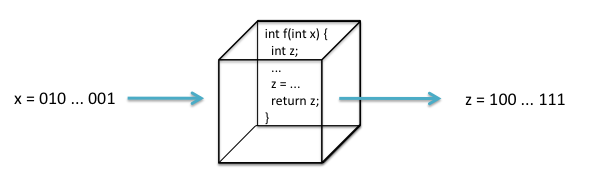
\includegraphics[width=0.8\textwidth]{computational_model_function}
    \caption{Caption for the figure.}
    \label{fig:fnCompModel}
\end{figure}

\begin{figure}[h] % Preferrably place figure here, not at the top/bottom of a page.
    \centering
    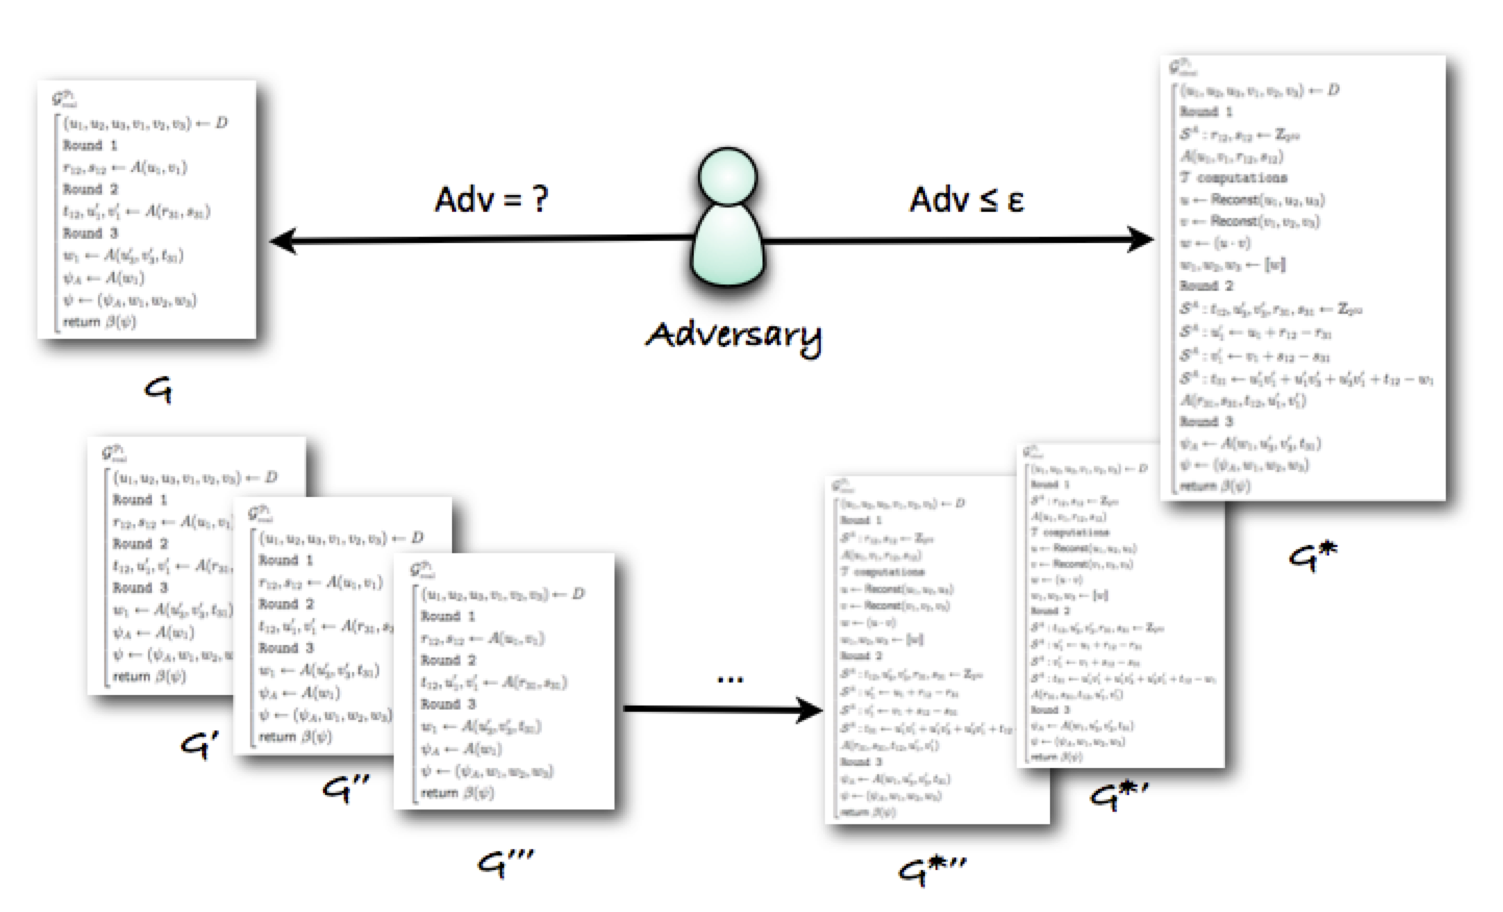
\includegraphics[width=\textwidth]{game-based_proofs}
    \caption{Cite if the figure is not yours~\cite{kamm12}.}
    \label{fig:game-based_proofs}
\end{figure}

\begin{figure}
    \centering
    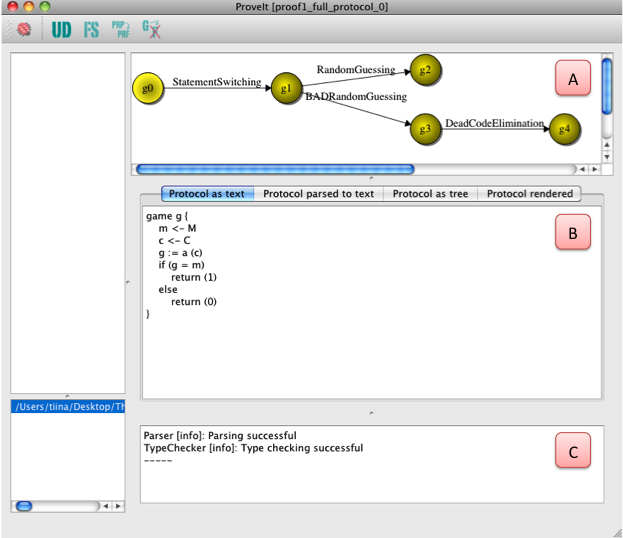
\includegraphics[width=\textwidth]{proveit_screenshot}
    \caption{Screenshot of \proveit.}
    \label{fig:proveit_screenshot}
\end{figure}

Tip: If you add a screenshot, then labeling the parts might help make the text more understandable (panel C vs bottom right part). For example:
A screenshot of \proveit can be seen in Figure~\ref{fig:proveit_screenshot}.
The user first enters the pseudocode of the initial game in panel~B.
\proveit also keeps track of all the previous games showing the progress on a graph shown in panel~A.

\begin{figure}
    \centering
    \begin{subfigure}[c]{0.45\textwidth}
        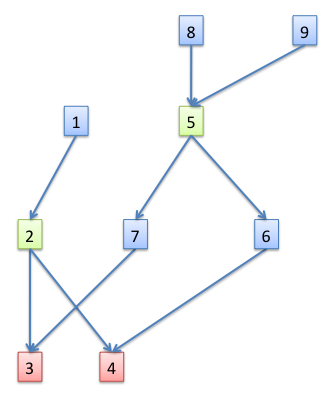
\includegraphics[width=\textwidth]{LCA_2_solutions}
        \caption{Example graph.}
        \label{fig:graph}
    \end{subfigure}
    \hfil % Add horizontal space between subfigures.
    \begin{subtable}[c]{0.3\textwidth}
        \centering
        \caption{Descendants per node.}
        \begin{tabular}{cl}
            \toprule
            Node & Decendants \\
            \midrule
            1 & 2, 3, 4 \\
            2 & 3, 4 \\
            3 & \\
            4 & \\
            5 & 3, 4, 6, 7 \\
            6 & 4 \\
            7 & 3 \\
            8 & 3, 4, 5, 6, 7\\
            9 & 3, 4, 5, 6, 7\\
            \bottomrule
        \end{tabular}
    \end{subtable}
    \caption{Example how to put two figures parallel to each other.}
    \label{fig:LCA_2_solutions}
\end{figure}

You can also use subfigures and subtables like in Figure~\ref{fig:LCA_2_solutions}.\footnote{Although you should avoid mixing subfigures and subtables like that.}


\subsection{Tables}

See Table~\ref{tab:statements} for an example of a nice and professional table that does not use vertical rules.
\TODO{Rule: Tables have captions above.}

\begin{table}
    \centering
    \caption{Statements in the \proveit language.}
    \label{tab:statements}
    \begin{tabular}{ll}
        \toprule
        Statement & Typeset Example \\
        \midrule
        assignment & $a := 5 + b$ \\
        uniform choice & $m \gets M$ \\
        function signature & $f : K \times M \to L$ \\
        \bottomrule
    \end{tabular}
\end{table}


\subsection{Lists}

Example of a numbered list:
\begin{enumerate}
    \item item one;
    \item item two;
    \item item three.
\end{enumerate}


\subsection{Math}

Variables or equations in text are surrounded by \verb|$| signs, e.g., $a$ and $x - y$.
This is a display equation:
\[
    x^2 + y^2 = z^2.
\]
This is a numbered equation:
\begin{equation}
    a + b = c + d.
    \label{eq:abcd}
\end{equation}
Multiple equations can be aligned like this:
\begin{align*} % The * means they are not numbered.
    a &= 5 \\
    b + c &= a \\
    a - 2 \cdot 3 &= \frac{5}{4}
\end{align*}


\subsection{Source code}

You can use the modern minted package to add highlighted source code like in Figure~\ref{fig:parser_exp}.

\begin{figure}
    \begin{minted}{antlr}
        expression
        : NUMBER
        | VARIABLE
        | '+' expression
        | expression '+' expression
        | expression '*' expression
        | function_name '(' parameters ')'
        | '(' expression ')'
    \end{minted}
    \caption{ANTLR grammar of arithmetic expressions.}
    \label{fig:parser_exp}
\end{figure}

\section{Conclusion}

\TODO{what did you do?}
\TODO{What are the results?}
\TODO{future work?}


% Bibliography
\clearpage % Flush all floats (figures and tables) before bibliography and start new page.
\nocite{*}
\printbibliography[heading=bibintoc] % Bibliography with heading also in Table of Contents.

% Appendices
\newpage
\begin{appendices}

\section{Glossary}
\label{app:glossary}

\printlicence % Licence

\end{appendices}

\end{document}
